\documentclass{beamer}
% September 2014 
% Author: Dr Rachid Hourizi and Dr. Michael Wright 
% Department of Computer Science, University of Bath
\usepackage{listings}
\usetheme{Boadilla} 
\usepackage{fixltx2e}
\usepackage{hyperref}
\lstset{language=Java}

\begin{document}

\begin{frame} 
\begin{center}
\textbf{Resources}
\end{center}
\begin{itemize}
\item More help with this course
\begin{itemize}
\item Moodle \url{http://moodle.bath.ac.uk/course/view.php?id=30475}
\item E-mail - programming1@lists.bath.ac.uk
\end{itemize}
\item Online C \alert{and Java} IDE
\begin{itemize}
\item \url{https://www.codechef.com/ide}
\item Remember to select Java from the drop down menu.
\end{itemize}
\end{itemize}
\end{frame}

\begin{frame} 
\begin{itemize}
\item The places that you can get additional support if you are finding the pace of the course a little fast now include
\begin{itemize}
\item \text{The A labs}
\item \text{One remaining B lab}
\item \text{The Drop in Sessions}
\end{itemize}
\item please note that some of the labs were previously scheduled at awkward times
\item to the (limited) extent that we could, we have rearranged the awkward labs in order to make them more accessible
\item please check the details on Moodle (and let us know if you cannot now get to a lab that you would otherwise have attended)
\end{itemize}
\end{frame}

\begin{frame}
\begin{itemize}
\item If you struggling with the exercises, pace of the course and/or coding in general
\item Please come and see Rachid or Michael
\end{itemize}
\end{frame}
 
\begin{frame} 
\begin{itemize}
\item If, on the other hand, you are finding the pace a little slow  
\item You can sign up for the Advanced Programming Labs
\bigskip
\item When and Where
\begin{itemize}
\item Friday 11.15 - 13.15 
\item EB 0.9
\end{itemize}
\end{itemize}
\end{frame}

\begin{frame}
\begin{center}
\textbf{Last Week}
\end{center}
\begin{itemize}
\item Complex Collections (In C)
\item Abstract Data Types (In C)
\end{itemize}
\end{frame}

\begin{frame}
\begin{center}
\textbf{This Week}
\end{center}
\begin{itemize}
\item First Objects (In Java)
\item Interacting Objects (In Java)
\item Short Feedback Session
\end{itemize}
\end{frame}

\begin{frame}{}
\begin{itemize}
\item This week marks a major turning point in the course
\begin{itemize}
\item We will move from using C
\item To using second programing language: Java
\end{itemize}
\end{itemize}\end{frame}\begin{frame}\begin{itemize}

\item That change means that you will have to learn
\begin{itemize}
\item new ways to write the instructions that we want the computer to execute and
\item a new way to think about the programs that we write whilst using
those instructions: Object Oriented Programming
\end{itemize}
\end{itemize}\end{frame}

\begin{frame}\begin{itemize}

\item As you make these changes, however, it is worth noting that you are
not starting from scratch

\begin{itemize}
\item When writing small Java programs, the programs that you write can appear reasonably
similar to those that you wrote in C
\item The Java version of HelloWorld, for example, bears some similarity
to the C version

\end{itemize}
\end{itemize}\end{frame}

\begin{frame}[fragile]
\begin{block}{}
\begin{lstlisting}
public class HelloWorld {

    public static void main(String[] args) {
        
	//print HelloWorld to the terminal
        System.out.println("Hello, World");
    }

}
\end{lstlisting}
\end{block}
\end{frame}

\begin{frame}\begin{itemize}

\item To some extent, you will also see similarities between 

\begin{itemize}
\item the ways in which you compile and run a Java program and
\item the ways in which you compile and run a C program
\end{itemize}
\item These similarities can be misleading, however

\begin{itemize}
\item On closer examination, the steps taken to prepare a Java program for
execution
\item Are different from those taken when preparing a C program
\end{itemize}
\end{itemize}\end{frame}

\begin{frame}
\frametitle{The Programming Language Java}
\begin{itemize}
\item The Java language is both compiled and
interpreted.  
\item Instead of translating Java programs into a 
machine language, the Java compiler generates Java byte code for its \alert{Virtual Machine}
\begin{itemize}
\item Byte code is easy (and fast) to interpret, like machine language,
\item but it is also portable, like a high-level language.  
\end{itemize}
\item Thus, it is possible to compile a Java program on one machine,
transfer the byte code to another machine over a network,
and then interpret the byte code on the other machine.  
\item This ability is one of the advantages of Java over many other
high-level languages.
\end{itemize}
\end{frame}

\begin{frame}[fragile]
\frametitle{Compiling and Running Simple a Program I}
\begin{itemize}
\item We can use compilation/interpetation of the HelloWorld program on an earlier slide as an example:
\item Before you start, the filename in which you save your main method should match the name of the class with the extension .java. In this case, HelloWorld.java
\item Note: Java is \alert{case sensitive}, just like C.
\end{itemize}
\end{frame}

\begin{frame}[fragile]
\frametitle{Compiling and Running a Simple Program II}
\begin{itemize}
\item To run the code:
\item we need to compile it: \lstinline!javac HelloPrinter.java!
\item This will generate a file \lstinline!HelloPrinter.class!, containing the virtual machine byte code
\item We can now run the code:
\end{itemize}
\begin{block}{}
\begin{lstlisting}
$javac HelloWorld.java
$java HelloWorld
Hello, World
\end{lstlisting}
\end{block}

\end{frame}

\begin{frame}[fragile]
\frametitle{Compiling and Running Programs Consisting of Multiple Classes}
\begin{itemize}
\item If you write a program involving multiple classes,
\item you would normally save each  class in a different file
\item Note: Each file must have a name of the form [classname].java
\item where [classname] is the name of the class contained in the file
\item If you have multiple files, you can compile tham all with one command. 
\item i.e. You can use \lstinline!javac *.java! to compile all .java files in the current directory in one go.
\item To run the program, you then need to use the interpreter command (\lstinline!java!) on the class that contains the \lstinline!main! method. 
\item We will return to multi-class programs later in the course
\begin{block}{}
\begin{lstlisting}
$javac *.java
$java HelloWorld
Hello, World
\end{lstlisting}
\end{block}
\end{itemize}
\end{frame}



\begin{frame}\begin{itemize}

\item Just as you did with C,

\item We would strongly suggest that you adopt an iterative approach to
developping Java programs i.e.

\begin{itemize}
\item start with a program that works 
\item (such as the Java version of HelloWorld introduced earlier)
\item and extend/debug it in small increments
\item until you have a program that does what you want
\end{itemize}
\end{itemize}\end{frame}\begin{frame}\begin{itemize}


\item In order to go beyond our HelloWorld program, however
\item You will need to understand that Java is an Object Oriented (OO) language
\item (Sometimes described as an Object Oriented Programming (OOP) language)
\bigskip
\bigskip
\item This begs two obvious questions:
\item What does it mean to be ``Object Oriented'' when
writing code?
\item And, in a programming context, what is an
Object anyway?
\end{itemize}
\end{frame}

\begin{frame}
\begin{itemize}
\item The (Data) Structures and Abstract Data Types (ADT's)
that we considered last week provide us with a useful starting point
when trying to understand Objects and Object Orientation.
\end{itemize}
\end{frame}

\begin{frame}
\begin{itemize}
\item The US National Institute of Standards and Technologies (NIST) starts
it's definition of a data structure as follows:

\begin{itemize}
\item An organization of information, usually in memory, for better algorithm
efficiency
\end{itemize}
\item By this definition, an Array is a data structure.
\item As we saw last week, an Array is an organisation (or organization)
of information in memory
\end{itemize}
\end{frame}


\begin{frame}\begin{itemize}
\item The NIST definition of an abstract data type is as follows:

\begin{itemize}
\item A set of data values and associated operations that are precisely
specified independent of any particular implementation
\end{itemize}
\end{itemize}\end{frame}\begin{frame}\begin{itemize}
\item It is useful to focus on two parts of this definition: 

\begin{itemize}
\item ``independent of any particular implementation'' 

\begin{itemize}
\item i.e. an abstract data type is defined once but can be implemented
in multiple ways
\end{itemize}
\item A set of data values and associated operations

\begin{itemize}
\item i.e. an abstract data type defines both data and operations
\end{itemize}
\end{itemize}
\end{itemize}\end{frame}

\begin{frame}\begin{itemize}
\item By this definition, a queue is a data type or collection 

\begin{itemize}
\item entities in the collection (values) are kept in order
\item and the principal (only?) operations on the collection are 

\begin{itemize}
\item the addition of entities to the rear
\item and removal of entities from the front 
\item (first in, last out)
\end{itemize}
\end{itemize}
\end{itemize}\end{frame}

\begin{frame}\begin{itemize}
\item Object Oriented Programming maintains this interest in associating
data with the operations that can be performed on it:
\item Object Oriented Programming: A type of programming in which programmers
define not only the data type of a data structure, but also the types
of operations (methods) that can be applied to the data structure.
In this way, the data structure becomes an object that includes both
data and functions.
\begin{itemize}
\tiny
\item http://www.webopedia.com/TERM/O/object\_oriented\_programming\_OOP.html
\normalsize
\end{itemize}
\end{itemize}\end{frame}\begin{frame}\begin{itemize}
\item C allowed us to use 
\begin{itemize}
\item data structures (Structs) and 
\item functions which allow us to manipulate those structures (Structs)
\end{itemize}
\item Java forces us to use 

\begin{itemize}
\item combinations of data structures and functions (\alert{Objects})

\begin{itemize}
\item some of which are pre-defined for us
\item and some of which we can define ourselves
\end{itemize}
\end{itemize}
\end{itemize}\end{frame}

\begin{frame}\begin{itemize}
\item Also, just as C allowed us to 

\begin{itemize}
\item define a data structure once 
\item and then create multiple examples of that structure
\end{itemize}
\item Java allows us to 
\begin{itemize}
\item define a combination of data and operations once (a \alert{Class})
\item and then create one or more examples (instances) of that class (\alert{Objects})
\end{itemize}
\end{itemize}\end{frame}

\begin{frame}\begin{itemize}
\item More accurately, each time we want to use a new combination of data
and operations, Java forces us to 

\begin{itemize}
\item start by defining a Class which combines that data and those operations
\item before creating one or more examples of that class (one or more Objects)
\end{itemize}
\item You can think of this process as 

\begin{itemize}
\item defining a template (the Class)
\item and using it to create one or more Objects using that template
\end{itemize}
\end{itemize}\end{frame}

\begin{frame}
\frametitle{Exercise}
\begin{tabular}{ll}
TelephoneNumber & lord-of-the-rings \\
BankAccount & Diary\\
harry-potter-and-the-Philosopher-Stone  & myDiary\\
01225-38-5053 & michaelWright\\
Book & Lecturer\\
rachidHourizi & myAccount\\
\end{tabular}
\end{frame}

\begin{frame}
\frametitle{Attributes and Fields}
\begin{itemize}
\item Just as C Structures contained values stored in member variables
\item an Object has \alert{attributes}: i.e. \alert{values} stored in \alert{fields}. (The data you encapsulate)
\item the class defines what fields an Object has, but each Object stores its own set of values.
The set of values stored in a single Object is called the \alert{state} of the object.
\end{itemize}
\end{frame}

\begin{frame}
\frametitle{State}
\begin{center}
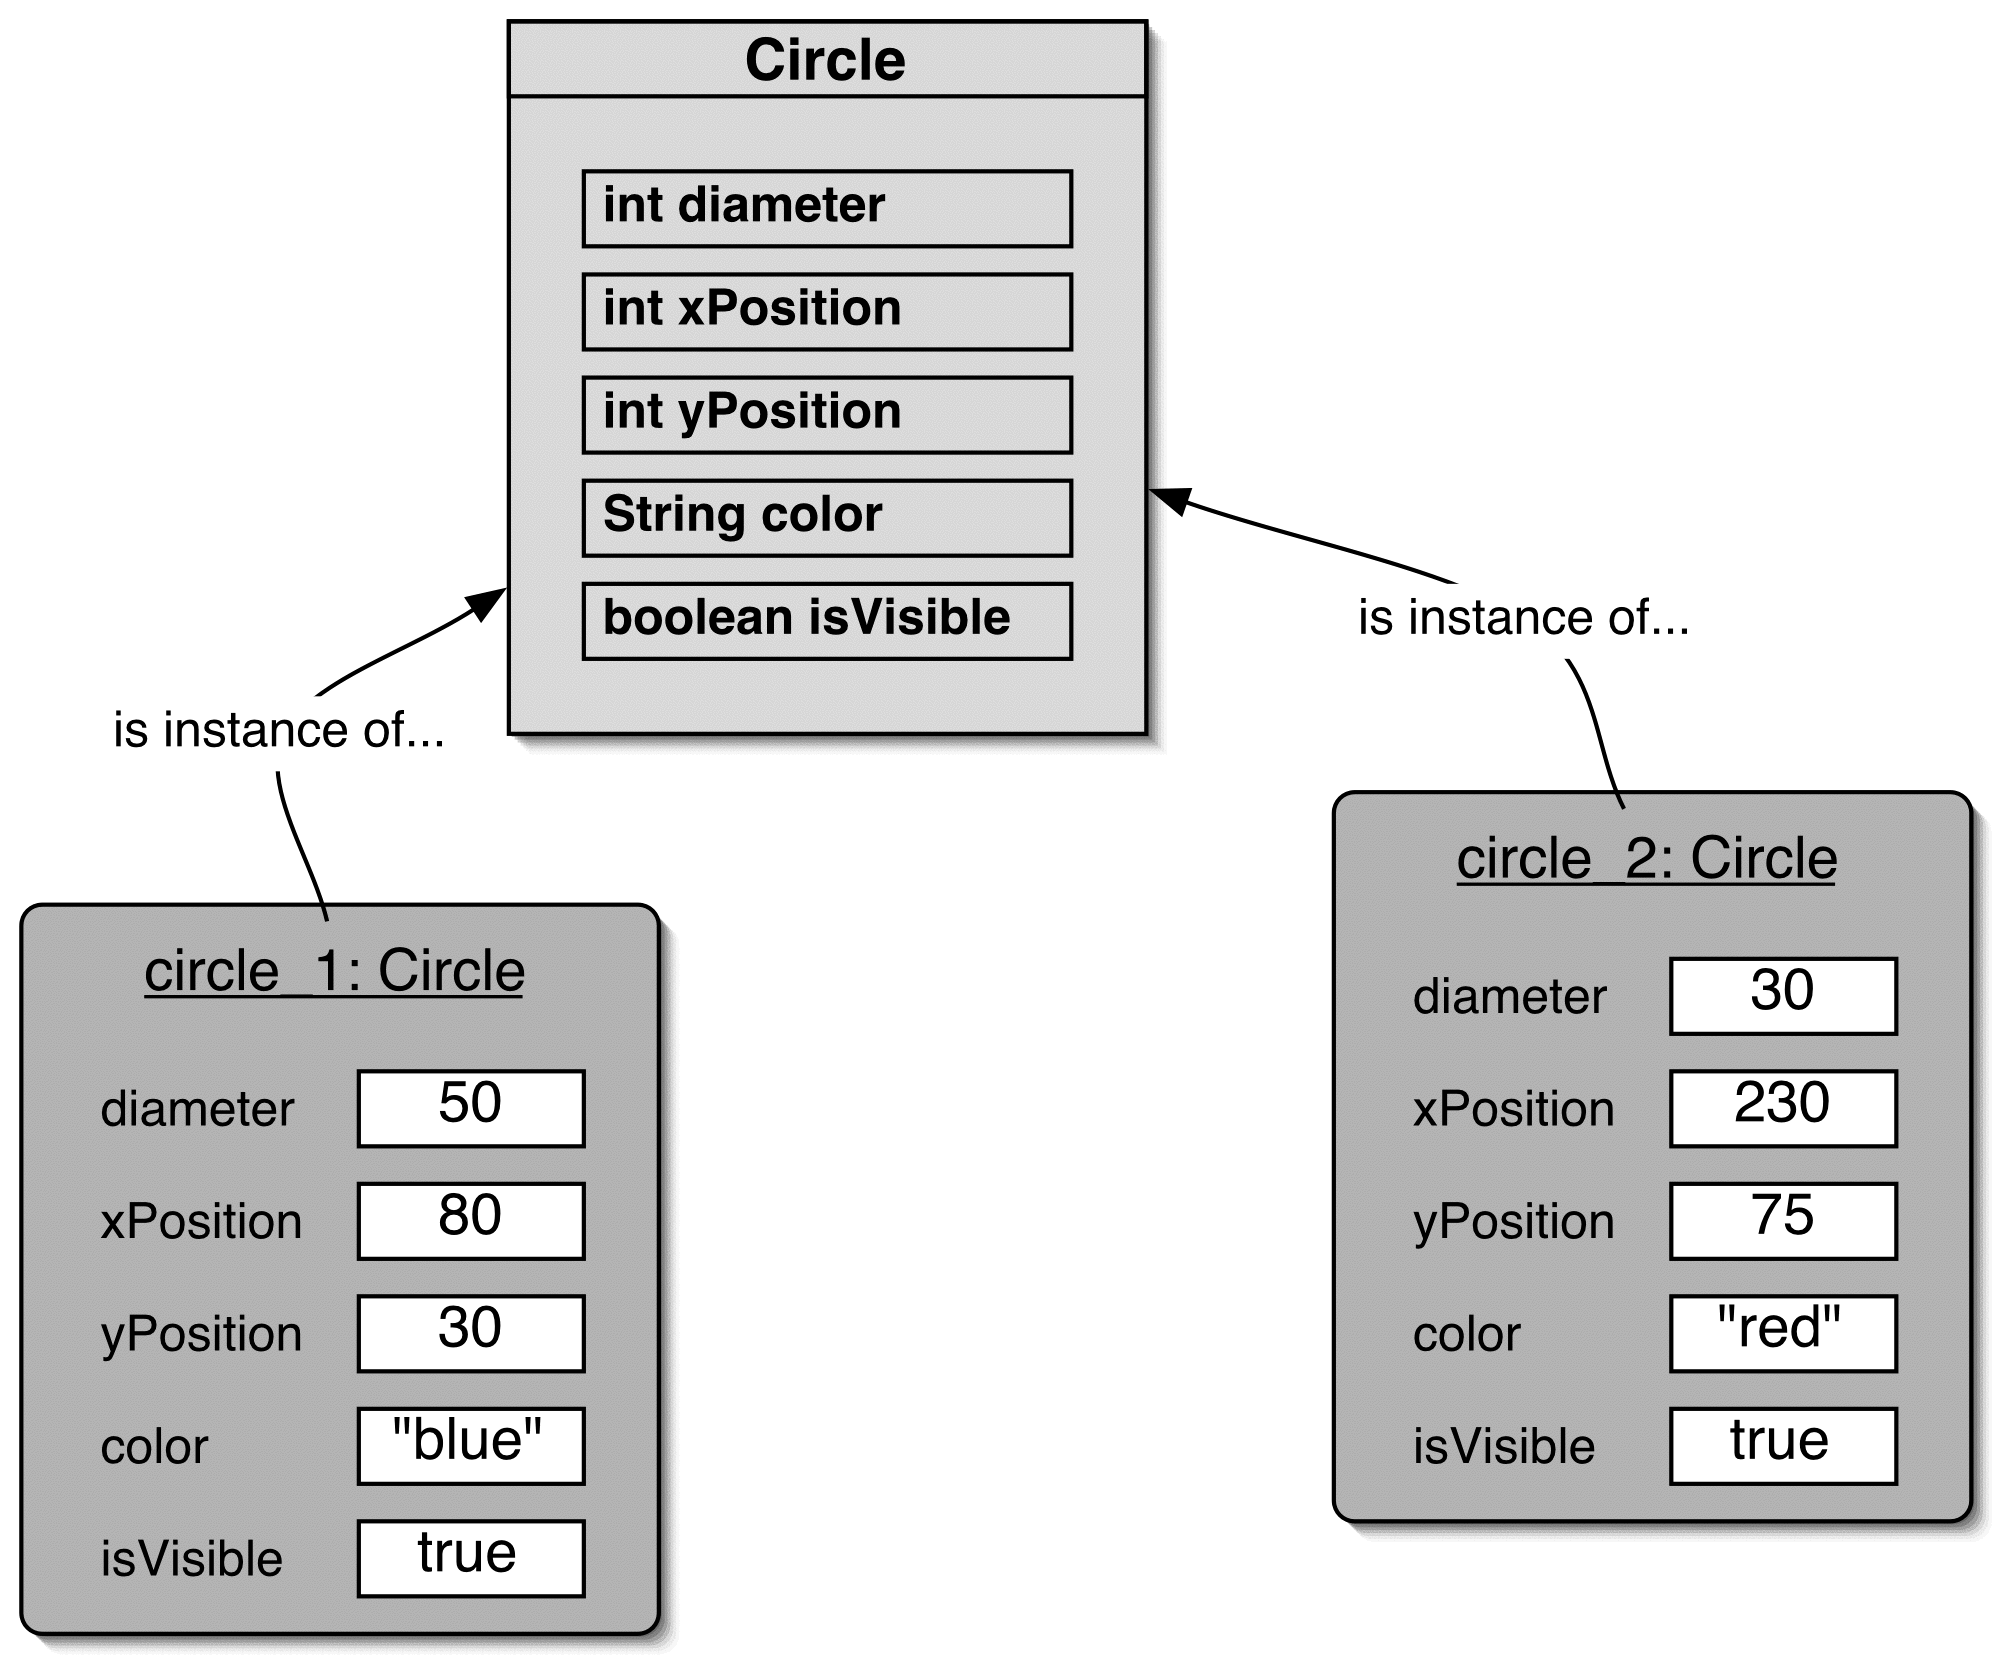
\includegraphics[height=5cm,keepaspectratio]{./figures/state}
\end{center}
\end{frame}


\begin{frame}[fragile]
\frametitle{Methods and Parameters}
\begin{itemize}
\item Objects/classes also have operations which can be invoked. They are called \alert{methods}
\item If, for example, we wanted to be able to
\begin{itemize}
\item draw examples of the circle class (Circle Objects) on screen and then
\item move those circles a specified distance to the right
\end{itemize}
\item we could include
\begin{itemize}
\item a drawCircle() method in our definition of the Circle class and
\item a moveRight() method in our definition of the Circle class
\end{itemize}
\end{itemize}
\begin{block}{}
\begin{lstlisting}
void moveRight(int distance){
	...some code...
}
\end{lstlisting}
\end{block}
\end{frame}

\begin{frame}
\begin{itemize}
\item The first piece of code used to implement a method e.g.  
\begin{itemize}
\item void moveRight(int distance)
\end{itemize}
\item provides a short description of what the method does
\item that short description is called the method's \alert{signature}
\item The collection of methods in a class is referred to as the \alert{interface} of that class
\end{itemize}
\end{frame}

\begin{frame}
\begin{itemize}
\item Methods are \alert{called} or \alert{invoked}
\item At the point of being called, they may need to recieve information as input if they are to perform the desired operation
\begin{itemize}
\item for example, our moveRight() method may need to be given a distance in order to move a Circle Object as intended
\end{itemize}
\item As in C, that information can be passed in the form of one or more \alert{parameters}
\item in the moveRight(int distance) example, int distance is an example a parameter
\end{itemize}
\end{frame}

\begin{frame}
\frametitle{Data Types}
\begin{itemize}
\item Both Fields and Parameters have \alert{types}. A type defines what kinds of values a parameter can take.
\item In Java (as in C) you have to specify the type.
\item e.g. we know that void moveRight(int distance) takes an integer as input because the distance parameter is defined as being of type int. 
\end{itemize}
\end{frame}

\begin{frame}
\begin{itemize}
\item In Java, everything has a type.
\item Examples of types: int, String, Circle, \ldots
\item Java is \alert{staticly typed language}
\item i.e. once you have given a field or parameter a type, that type cannot change
\item Note: Each time you create a new class, you have defined a new type
\end{itemize}
\end{frame}

\begin{frame}
\frametitle{Source Code}
\begin{itemize}
\item Each class has source code associated with it that defines its details (fields and methods).
\item The code defining each class determines the structure and the behavior of each of its instances (i.e. the structure and behaviour of each Object created using the class template).
\item This source code is compiled and interpreted by Java.
\end{itemize}
\end{frame}

\begin{frame}
\frametitle{Return Values}
\begin{itemize}
\item Methods may return a result via a \alert{return value}.
\item Example: \lstinline!String getName()‏!
This method returns a String.
\item Example: \lstinline!void changeName()‏!
\alert{Void} indicates that this method does not return anything
\end{itemize}
\end{frame}

\begin{frame}
\frametitle{Developing Java Programs}
\begin{itemize}
\item To learn to develop Java programs, one needs to learn how to write class definitions, including fields and methods, and how to put these classes together
\item We will look at these issues in more detail during the remainder of this course
\end{itemize}
\end{frame}

\begin{frame}
\frametitle{Coding Conventions}
\begin{itemize}
\item Classes: Uppercase to start, merge words, consecutive words uppercase, nouns
E.g. Car, Number, BankAccount
\item Objects: Lowercase to start, merge words, consecutive words uppercase, nouns
E.g. myBlueCar, Rational
\item Methods: Lowercase to start, merge words, consecutive words uppercase, verbs
E.g. moveLocation, deposit
\end{itemize}
\end{frame}

\begin{frame}
\frametitle{Ticket Machines – An External/User View}
Exploring the behaviour of a typical ticket machine.
\begin{itemize}
\item Use the naive-ticket-machine project.
\item Machines supply tickets of a fixed price.
\item How is that price determined?
\item How is ‘money’ entered into a machine?
\item How does a machine keep track of the money that is entered?
\item How is a ticket provided?
\end{itemize}
\end{frame}

\begin{frame}[fragile]
\frametitle{Ticket Machine Fields and Initial State}
\begin{lstlisting}[linewidth=5cm]

public class TicketMachine
{
private int price = 500;
private int balance = 0;
private int total = 0;

... more code

}
\end{lstlisting}
\end{frame}


\begin{frame}[fragile]
\frametitle{Ticket Machine Methods: The Interface}
\begin{lstlisting}[linewidth=7cm]
public class TicketMachine
{

... fields....

public int getBalance()
public int getPrice()
public void insertMoney()
public void printTicket()

...more code

}

\end{lstlisting}
\end{frame}

\begin{frame}
\frametitle{Ticket Machines – An Internal/Programmer view}
\begin{itemize}
\item Interacting with an object gives us clues about its behavior.
\item Looking at the source code allows us to determine how that behavior is provided or implemented.
\item There is a recognised structure to the source code associated with each class.
\end{itemize}
\end{frame}

\begin{frame}[fragile]
\frametitle{TicketMachine Source Code}
\tiny
\begin{lstlisting}
/**
 * TicketMachine models a naive ticket machine that issues
 * flat-fare tickets.
 * The price of a ticket is specified via the constructor.
 * It is a naive machine in the sense that it trusts its users
 * to insert enough money before trying to print a ticket.
 * It also assumes that users enter sensible amounts.
 *
 * @author David J. Barnes and Michael Kolling
 * @version 2002.02.06
 */
public class TicketMachine
{
    // The price of a ticket from this machine.
    private int price;
    // The amount of money entered by a customer so far.
    private int balance;
    // The total amount of money collected by this machine.
    private int total;


    //continued on next slide
\end{lstlisting}
\end{frame}

\begin{frame}[fragile]
\tiny
\begin{lstlisting}

    //continued from previous slide

    /**
     * Create a machine that issues tickets of the given price.
     * Note that the price must be greater than zero, and there
     * are no checks to ensure this.
     */
    public TicketMachine(int ticketCost)
    {
        price = ticketCost;
        balance = 0;
        total = 0;
    }

    //continued on next slide
\end{lstlisting}
\end{frame}

\begin{frame}[fragile]
\tiny
\begin{lstlisting}

    //continued from previous slide

    /**
     * Return the price of a ticket.
     */
    public int getPrice()
    {
        return price;
    }
}
\end{lstlisting}
\end{frame}

\begin{frame}[fragile]
\frametitle{Basic class structure}
\begin{lstlisting}
public class TicketMachine
{
    Inner part of 
    the class omitted.
}
\end{lstlisting}
\end{frame}

\begin{frame}[fragile]
\frametitle{Basic class structure}
\begin{lstlisting}
public class ClassName
{
    Fields
    Constructors
    Methods
} 
\end{lstlisting}
\end{frame}

\begin{frame}
\frametitle{Comments/Documentation}
\begin{itemize}
\item As with C, Comments make Java source code easier to read for humans. No effect on the functionality.
\item Three sorts:
\begin{itemize}
\item \lstinline!// comment!: single-line comments
\item \lstinline!/* comments */!: multiple-lines – more detail
\item \lstinline!/** */!: similar to previous, but used when documentation software is used.
\end{itemize}
\end{itemize}
\end{frame}

\begin{frame}[fragile]
\frametitle{Fields}
Recap:
\begin{itemize}
\item \alert{Fields} store values for an object.
\item They are also known as \alert{instance variables}.
\item Fields define the \alert{state} of an object.
\item Fields have an associated \alert{type}.
\end{itemize}

\begin{lstlisting}
public class TicketMachine
{
    private int price;
    private int balance;
    private int total;
 
    Constructor and methods omitted.
} 
\end{lstlisting}
\end{frame}

\begin{frame}[fragile]
\frametitle{Constructors}
\begin{itemize}
\item Constructors create and initialize an object.
\item Then assign the necessary memory to the created object
\item They have the same name as their class.
\item They store initial values into the fields.
\item They often receive external parameter values for this.
\end{itemize}

\begin{lstlisting}
public TicketMachine(int ticketCost)‏
{
    price = ticketCost;
    balance = 0;
    total = 0;
} 
\end{lstlisting}
\end{frame}

\begin{frame}[fragile]
\frametitle{Creating Objects}
\begin{itemize}
\item Constructors are used to create and initialise a new object
\tiny
\begin{lstlisting}

public class TrainSimulator {

    public static void main(String[] args) {
        
	//create a new TicketMachine Object and store it in the variable machine
        TicketMachine machine = new TicketMachine(500);
    }

}


\end{lstlisting}
\item This creates a new TicketMachine object and stores it in a variable named machine which is
of type TicketMachine.
\end{itemize}
\end{frame}

\begin{frame}[fragile]
\frametitle{Parameters}
\begin{itemize}
\item Parameter names inside a constructor or method are referred to as \alert{Formal Parameters}
\item Parameter values provided from the outside are referred to as \alert{Actual Parameters}.
\item In the constructor \lstinline!TicketMachine(int ticketCost)! 
\item ticketCost is a 
formal parameter. 
\item When the constructor is called, using \lstinline!TicketMachine(500)!, 
\item 500 is an actual parameter.
\end{itemize}
\end{frame}

\begin{frame}
\frametitle{Scope and Lifetime}
\begin{itemize}
\item The \alert{scope} of a variable/parameter defines the section of the code from which it can be accessed.
\item For instance variables (fields) this is the entire class.
\item For parameters, this is the constructor or method that declares it. 
\item Trick: find the enclosing \{\}, this is the scope. 
\item The \alert{lifetime} of a variable/parameter describes how long the variable continues to exist before it is destroyed.
\end{itemize}
\end{frame}

\begin{frame}[fragile]
\frametitle{Assignment}
\begin{itemize}
\item Similar to C:
\item Values are stored into fields (and other variables) via \alert{assignment} statements:
\begin{itemize}
\item \lstinline!variable = expression;!
\item e.g. \lstinline!price = ticketCost;!
\end{itemize}
\item Both sides of the assignment should have the same type, e.g. int, double, String, TicketMachine, ...
\item A variable stores a single value, so (as in C) any previous value is lost after an assignment.
\end{itemize}
\end{frame}


\begin{frame}[fragile]
\frametitle{Accessor Methods I}
\begin{itemize}
\item All methods implement object behaviour.
\item And all methods have a structure consisting of a header and a body.
\item The header defines the \alert{method’s signature} e.g.   
\begin{lstlisting}
   public int getPrice()‏{
	
	... method body ...

   }

 
\end{lstlisting}

\item The body encloses the method’s statements e.g.
\end{itemize}
\begin{lstlisting}
      ... header{

	   return price;

      }
\end{lstlisting}
\end{frame}

\begin{frame}[fragile]
\begin{itemize}
\item We can, however, be more precise about the kind of behaviour implemented by particular methods
\item \alert{Accessors}, for example are methods which provide information about an object.
\item i.e. they allow users, other programs or other parts of your program to gain information about an object's state
\end{itemize}
\begin{lstlisting}
   public int getPrice()‏
   {
       return price;
   } 
\end{lstlisting}
\end{frame}

\begin{frame}
\frametitle{Mutator Methods}
\begin{itemize}
\item \alert{Mutators} have a similar method structure: header and body.
\item Used to \alert{mutate} (i.e., change) an object’s state.
\item Achieved through changing the value of one or more fields.
\begin{itemize}
\item Typically receive parameters.
\item Typically contain assignment statements.
\end{itemize}
\end{itemize}
\end{frame}

\begin{frame}[fragile]
\frametitle{Mutator methods}
\begin{lstlisting}
public void insertMoney(int amount)‏
{
    balance += amount;
} 
\end{lstlisting}
\end{frame}

\begin{frame}
\frametitle{Data Types}
\begin{itemize}
\item As we have seen in the code examples above, Java (like C) provides us with common data types 
\item e.g. integers: 
\begin{itemize}
\item int distance =7;
\end{itemize}
\item you won't be surprised to learn that Java also provides us with chars
\begin{itemize}
\item char myChar ='c';
\end{itemize}
\item and with booleans
\begin{itemize}
\item boolean a = false; 
\end{itemize}
\end{itemize} 
\end{frame}

\begin{frame}
\frametitle{Data Types}
\begin{itemize}
\item Java also provides us with ways to implement Strings and Arrays
\item We will return to these data types
\item ..but for now be a little careful with them
\item ..Java and C treat them in rather different ways
\end{itemize} 
\end{frame}

\begin{frame}
\begin{itemize}
\item Each time that we define a class, however, we define a new data type
\item Can be used as parameter, field and return types
\item The internal is hidden from the user
\begin{itemize}
\item No direct access to fields (unless special reason)‏
\item Access to state via accessor and mutator methods
\end{itemize}
\item User does not need to know how the class is implemented to use/instantiate it
\item The usage of a class is defined by its methods
\end{itemize}
\end{frame}

\begin{frame}[fragile]
\frametitle{Printing from methods}
\begin{lstlisting}
public void printTicket()‏
{
    // Simulate the printing of a ticket.
    System.out.println("##################");
    System.out.println("# The BlueJ Line");
    System.out.println("# Ticket");
    System.out.println("# " + price + " cents.");
    System.out.println("##################");
    System.out.println();
 
    // Update the total collected with the balance.
    total += balance;
    // Clear the balance.
    balance = 0;
} 
\end{lstlisting}
\end{frame}

\begin{frame}
\frametitle{Output}
\begin{center}
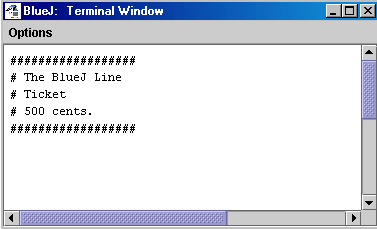
\includegraphics[height=5cm, keepaspectratio]{./figures/ticketOut}
\end{center}
\end{frame}

\begin{frame}
\frametitle{Reflecting on the ticket machines}
\begin{itemize}
\item Our first implementation of a TicketMachine class provides some useful functionality
\item But the behaviour of the TicketMachine objects we create using that class is inadequate in several ways:
\begin{itemize}
\item No checks on the amounts entered.
\item No refunds.
\item No checks for a sensible initialization.
\end{itemize}
\item How can we do better?
\begin{itemize}
\item We need more sophisticated behaviour.
\end{itemize}
\end{itemize}
\end{frame}

\begin{frame}[fragile]
\begin{itemize}
\item We can use conditionals to make choices in our Java code (Just as we did in C)
\end{itemize}
\small
\begin{lstlisting}
   public void insertMoney(int amount)‏
   {
       if(amount > 0) {
           balance += amount;
       }
       else {
           System.out.println("Use a positive amount: " +
                              amount);
       }
   }
\end{lstlisting}
\end{frame} 

\begin{frame}[fragile]
\frametitle{Making choices}
\small
\begin{lstlisting}
if(perform some test) {
    Do the statements here if the test gave a true result
}
else {
    Do the statements here if the test gave a false result
} 
\end{lstlisting}
\end{frame}

\begin{frame}
\frametitle{Coding Convention}
\begin{itemize}
\item If statement
\begin{itemize}
\item Always use \{ , even if there is only one statement
\item In case there is an else statement, start on a new line and use \{
\end{itemize}
\item Indentation
\begin{itemize}
\item Always indent your code, even if your text editor does not do it automatically
\end{itemize}
\item Document your code, the sooner the better. 
\end{itemize}
\end{frame}

\begin{frame}[fragile]
\frametitle{Boolean Tests}
\begin{itemize}
\item{$==$} : equality
\item{$>$} : greater than
\item{$<$} : less than
\item{$<=$} : less or equal than
\item{$>=$} : greater or equal than
\item{$!=$} : not equal
\end{itemize}
\end{frame}

\begin{frame}
\frametitle{Local variables}
\begin{itemize}
\item Fields are one sort of variable.
\begin{itemize}
\item They store values through the life of an object.
\item They are accessible throughout the class.
\item A bit like global variables in C
\end{itemize}
\item Methods can include shorter-lived variables.
\begin{itemize}
\item They exist only as long as the method is being executed.
\item They are only accessible from within the method.
\item Like function variables in C
\end{itemize}
\end{itemize}
\end{frame}

\begin{frame}[fragile]
\frametitle{Local variables}
\begin{lstlisting}
public int refundBalance()‏
{
    int amountToRefund;
    amountToRefund = balance;
    balance = 0;
    return amountToRefund;
} 
\end{lstlisting}
\end{frame}

\begin{frame}
\frametitle{Review}
\begin{itemize}
\item Class bodies contain fields, constructors and methods.
\item Fields store values that determine an object’s state.
\item Constructors initialize objects.
\item Methods implement the behaviour of objects.
\item Mutators (mutator methods) change the state of a object
\item Accessors (accessor methods) provide information about the state of an object 
\end{itemize}
\end{frame}

\begin{frame}
\frametitle{Review}
\begin{itemize}
\item Fields, parameters and local variables are all variables.
\item Fields persist for the lifetime of an object.
\item Parameters are used to receive values into a constructor or method.
\item Local variables are used for short-lived temporary storage. 
\item Objects can make decisions via conditional (if) statements.
\item A true or false test allows one of two alternative courses of actions to be taken.
\end{itemize}
\end{frame}

\begin{frame}
\frametitle{A digital clock}
\begin{center}
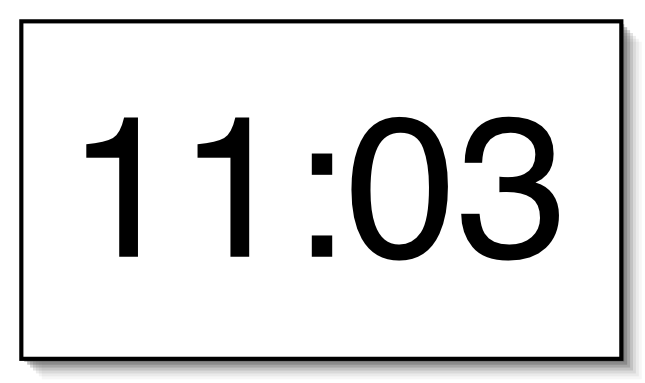
\includegraphics[height=5cm,keepaspectratio]{./figures/clock}
\end{center}
\end{frame}

\begin{frame}
\frametitle{Abstraction and modularization}
\begin{itemize}
\item \alert{Abstraction} is the ability to ignore details of parts to focus attention on a higher level of a problem. 
\item \alert{Modularization} is the process of dividing a whole into well-defined parts, which can be built and examined separately, and which interact in well-defined ways. 
\end{itemize}
\end{frame}

\begin{frame}
\frametitle{Modularizing the clock display}
\begin{tabular}{lll}
\begin{minipage}{3cm}
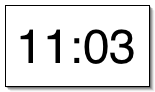
\includegraphics[height=1cm,keepaspectratio]{./figures/cl1} \end{minipage} & \mbox{}\hspace{1cm} & One four-digit display?\\
\mbox{}\\
\begin{minipage}{3cm}
Or two two-digit displays
\end{minipage}& & \begin{minipage}{3cm}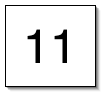
\includegraphics[height=1cm,keepaspectratio]{./figures/cl2}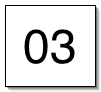
\includegraphics[height=1cm,keepaspectratio]{./figures/cl3}\end{minipage}
\end{tabular}
\end{frame}

\begin{frame}[fragile]
\frametitle{Implementation: NumberDisplay}
\begin{lstlisting}
public class NumberDisplay
{
    private int limit;
    private int value;

    Constructor and
    methods omitted.
}
\end{lstlisting}
\end{frame}

\begin{frame}[fragile]
\frametitle{Implementation: ClockDisplay}
\begin{lstlisting}
public class ClockDisplay
{
    private NumberDisplay hours;
    private NumberDisplay minutes;

    Constructor and
    methods omitted.
}
\end{lstlisting}
\end{frame}

\begin{frame}
\frametitle{Object diagram}
\begin{center}
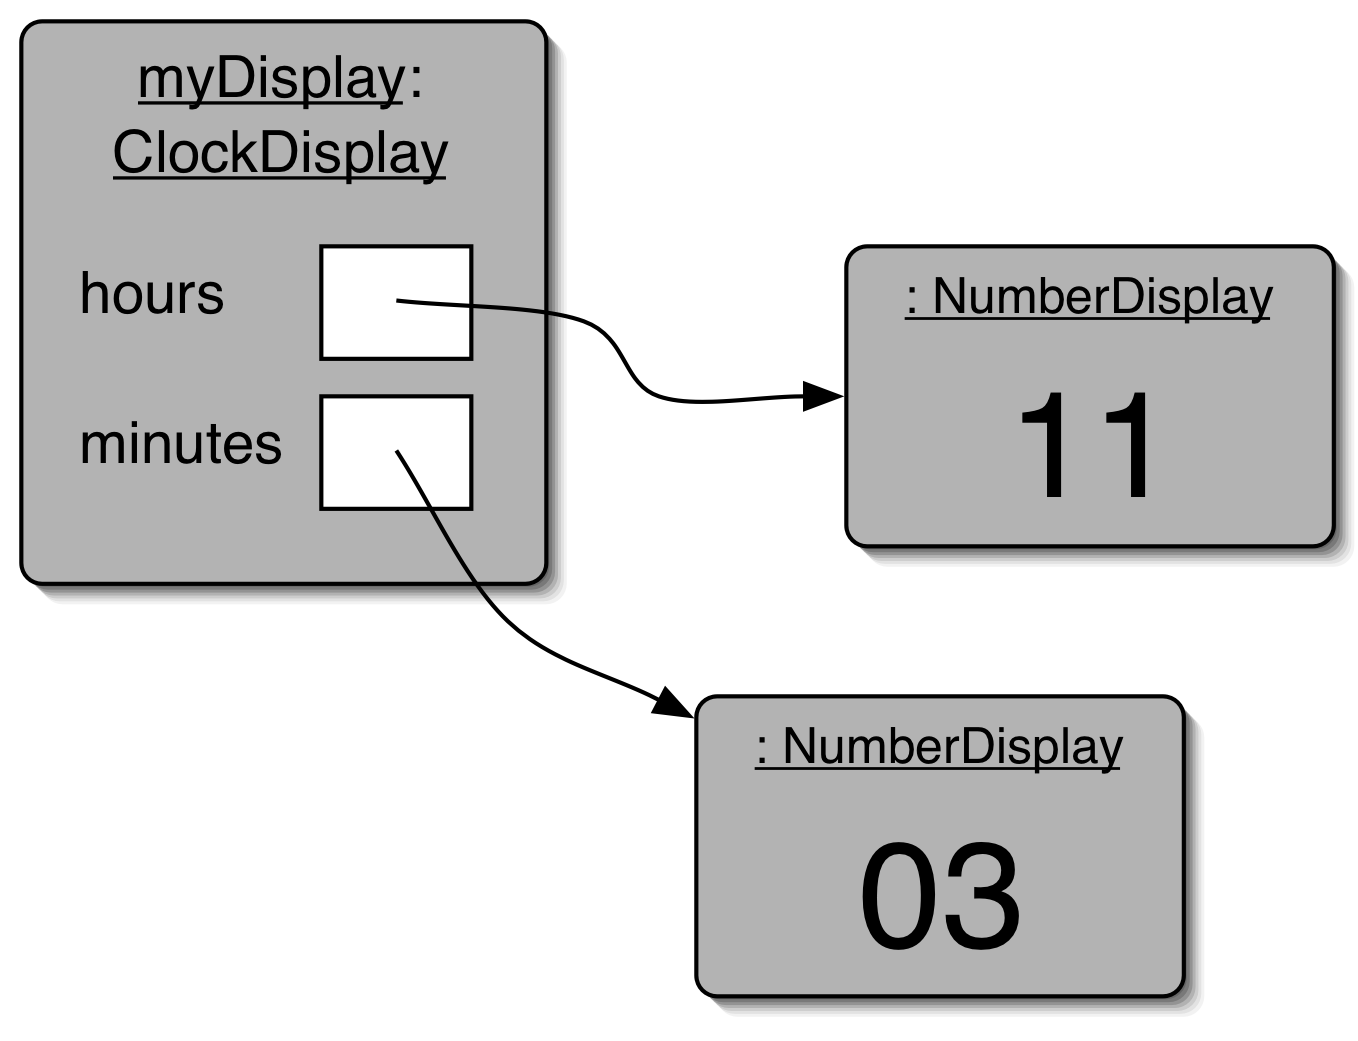
\includegraphics[height=5cm, keepaspectratio]{./figures/object}
\end{center}
\end{frame}

\begin{frame}
\frametitle{Class diagram}
\begin{center}
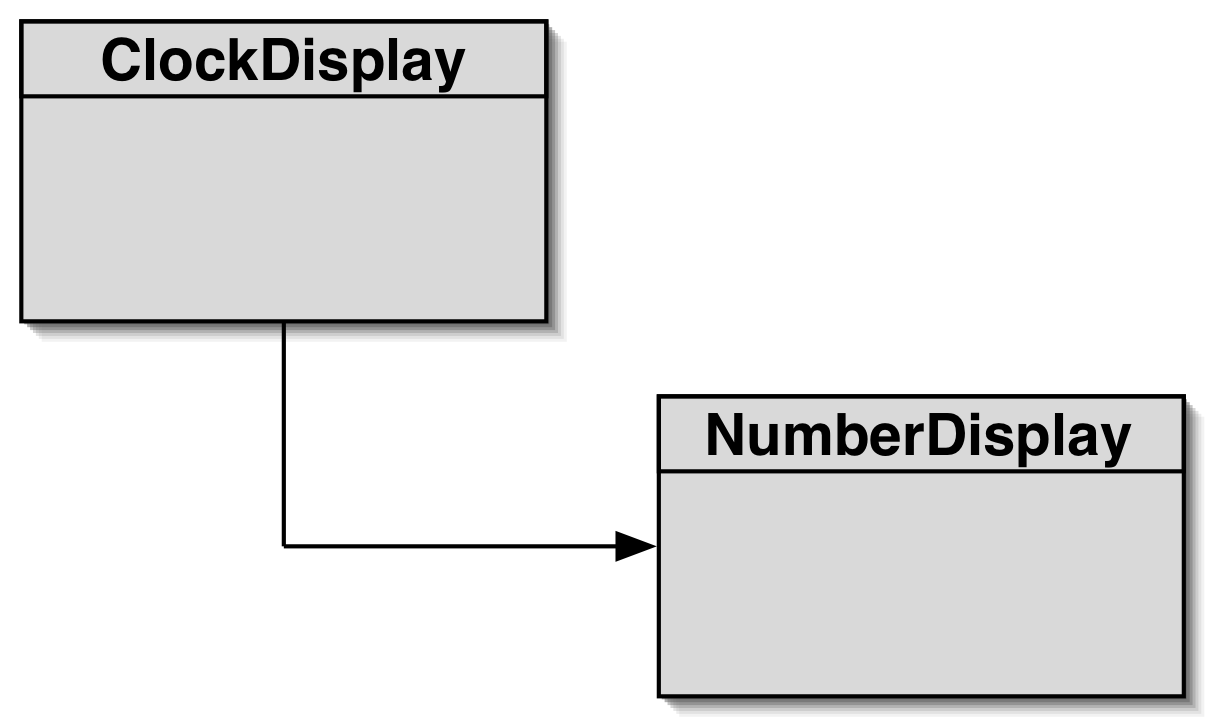
\includegraphics[height=5cm, keepaspectratio]{./figures/class}
\end{center}
\end{frame}

\begin{frame}
\frametitle{Diagrams}
\begin{itemize}
\item Class Diagrams
\begin{itemize}
\item Shows the classes of an application and the relationships between them
\item Gives information about the source code
\item Static view of the program
\end{itemize}
\item Object Diagrams
\begin{itemize}
\item Shows objects and their relationships at one moment in time during the execution of the program
\item Dynamic view of the program
\end{itemize}
\end{itemize}
\end{frame}

\begin{frame}
\frametitle{Primitive types vs. object types}
\begin{itemize}
\item Java defines two very different kinds of type: primitive types and object types.
\item Primitive types are predefined by Java.
\item Object types originate from classes.
\item Variables and parameters store references to objects.
\item The primitive types are non-object types.
\item This is the reason why Java is not a completely object oriented languages
\end{itemize}
\end{frame}

\begin{frame}
\frametitle{Call-by-reference and Call-by-value}
\begin{itemize}
\item There are two ways of passing arguments to methods in many programming languages: call-by-value and call-by-reference.
\item Call-by-value: A copy of the actual parameter is passed to the formal parameter of the called method. Any change made to the formal parameter will have no effect on the actual parameter.
\item Call-by-reference: the caller gives the called method the ability to directly access to the caller’s data and to modify that data if the called method so chooses.
\item Just like C Java uses call-by-value
\item For objects, the value is a reference to memory (like in C)
\end{itemize}
\end{frame}

\begin{frame}[fragile]
\frametitle{Source code: NumberDisplay}
\begin{lstlisting}
public class NumberDisplay
{
    private int limit;
    private int value;

          public NumberDisplay(int rollOverLimit)‏
{
    limit = rollOverLimit;
    value = 0;
}
\end{lstlisting}
\end{frame}

\begin{frame}[fragile]
\frametitle{Source code: NumberDisplay}
\begin{lstlisting}
public int getValue()‏
    {
        return value;
    }

public void setValue(int replacementValue)‏
    {
        if((replacementValue >= 0) && 
           (replacementValue < limit))‏
            value = replacementValue;
    }
\end{lstlisting}
\end{frame}

\begin{frame}
\frametitle{Logical Operators}
\begin{itemize}
\item \&\& : and, operands are tested, left to right, until conclusion can be reached 
\item $\mid \mid$ : or, operands are tested, left to right, until conclusion can be reached
\item ! : not
\item \& : and, both operands are tested
\item $\mid$ : or, both operands are tested
\end{itemize}
\end{frame}

\begin{frame}[fragile]
\frametitle{Source code: NumberDisplay}
\begin{lstlisting}
public String getDisplayValue()‏
{
    if(value < 10)‏
        return "0" + value;
    else
        return "" + value;
}

public void increment()‏
    {
        value = (value + 1) % limit;
    }
\end{lstlisting}
\end{frame}

\begin{frame}
\frametitle{String Concatenation}
\begin{itemize}
\item Addition:
\begin{itemize}
\item 12 + 24
\end{itemize}
\item String Concatenation:
\begin{itemize}
\item ``Java'' + `` and C'' $->$ ``Java and C''
\item ``answer': '' + 42 $->$ ''answer: 42''
\end{itemize}
\end{itemize}
\end{frame}

\begin{frame}[fragile]
\frametitle{String toString() method}
\begin{itemize}
\item String toString() method: Java provides a way of transforming every Object into a String. 
\item To tailor this to your own preference write a method toString() returning a String representation of your class/object.
\begin{lstlisting}
public String toString()‏
{
	return ``value: '' + value + `` with limit '' + limit;
}
\end{lstlisting}
\end{itemize}
\end{frame}

\begin{frame}
\frametitle{The Modulo Operator}
\begin{itemize}
\item \% : the modulo operator calculates the remainder of an integer division
\begin{itemize}
\item 27 \% 4 $->$ 3
\end{itemize}
\item Division in Java: if both arguments are integers, division will result in an integer.
\begin{itemize}
\item double res = 5 / 2 $->$ res = 2
\item double res = 5 / (2.0) or 5 / (2 * 1.0)    $->$ res = 2.5
\end{itemize}
\end{itemize}
\end{frame}

\begin{frame}[fragile]
\frametitle{Objects creating objects}
\begin{lstlisting}
public class ClockDisplay
{
    private NumberDisplay hours;
    private NumberDisplay minutes;
    private String displayString; 
    
    public ClockDisplay()‏
    {
        hours = new NumberDisplay(24);
        minutes = new NumberDisplay(60);
        updateDisplay();
    }
}
\end{lstlisting}
\end{frame}

\begin{frame}
\frametitle{Objects creating objects}
\begin{enumerate}
\item new ClassName(parameter-list)‏
\begin{itemize}
\item It creates a new object of the named class
\begin{itemize}
\item here NumberDisplay
\item this involves creating sufficient memory to store the values of primitive instance variables and references to object instance variables.
\end{itemize}
\end{itemize}
\item It executes the constructor of that class
\end{enumerate}
\end{frame}

\begin{frame} 
\frametitle{ClockDisplay object diagram}
\begin{center}
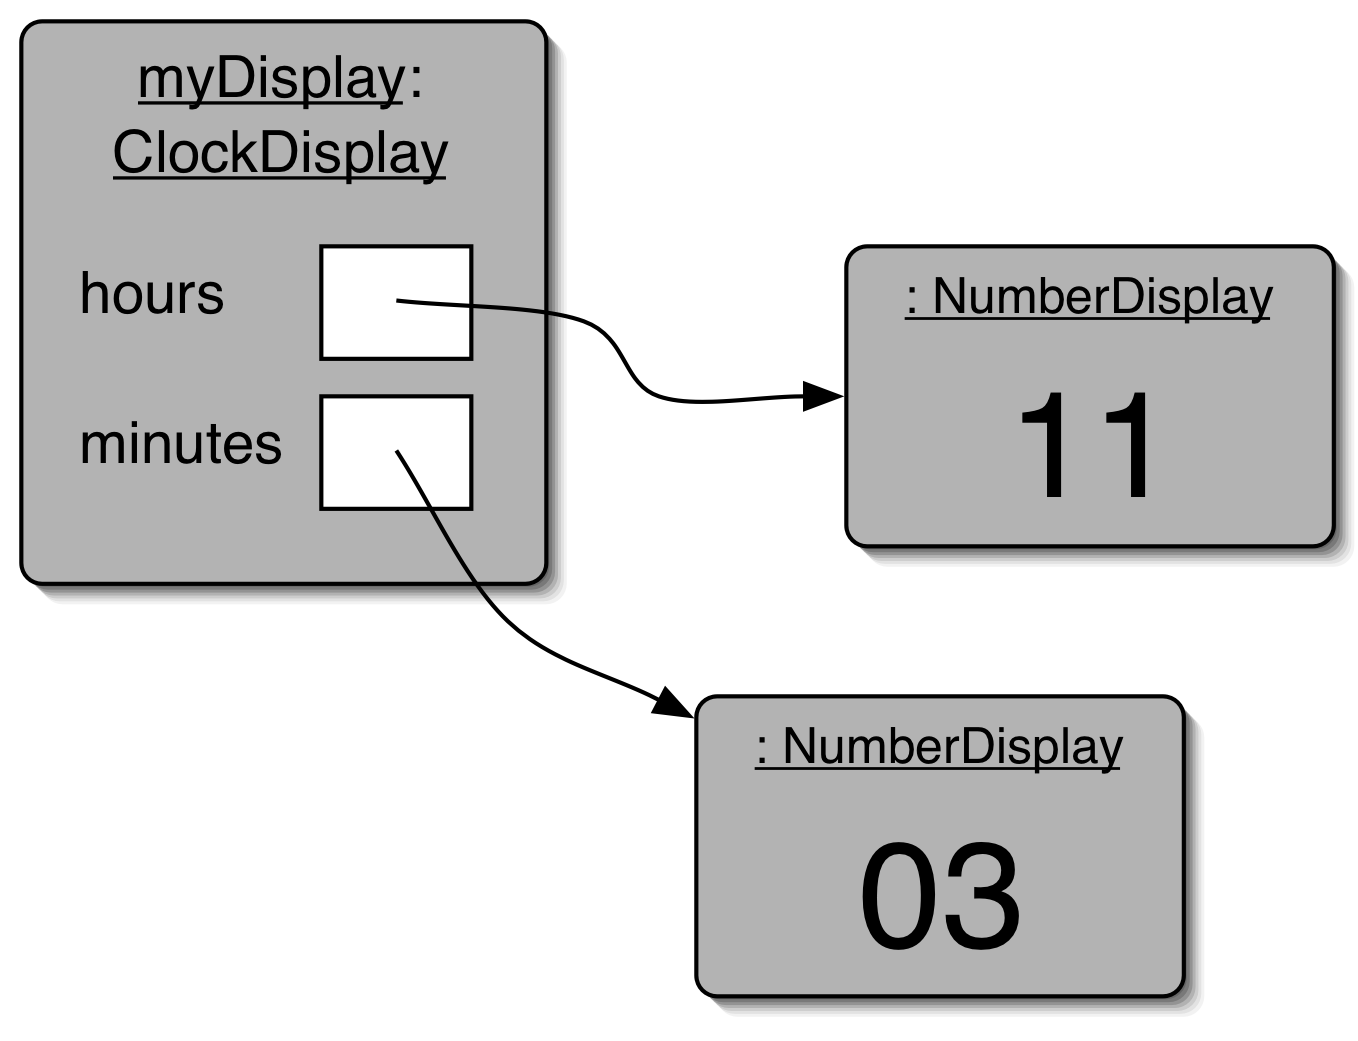
\includegraphics[height=5cm, keepaspectratio]{./figures/object}
\end{center}
\end{frame}


\begin{frame}
\frametitle{Method Overloading}
\begin{itemize}
\item Multiple Constructors of ClockDisplay:
\begin{itemize}
\item \lstinline!new Clockdisplay()‏!
\item \lstinline!new Clockdisplay(hour, minute)‏!
\end{itemize}
\item It is common for class definitions to contain alternative versions of constuctors or methods that provide various ways of achieving a particular task via their distinctive sets of parameters.
\item This is known as \alert{overloading}.
\end{itemize}
\end{frame}

\begin{frame}[fragile]
\frametitle{Method calling}
\begin{lstlisting}
public void timeTick()‏
{
    minutes.increment();
    if(minutes.getValue() == 0) { 
        // it just rolled over!
        hours.increment();
    }
    updateDisplay();
}
\end{lstlisting}
\end{frame}

\begin{frame}[fragile]
\frametitle{Internal method}
\begin{lstlisting}
/**
 * Update the internal string that
 * represents the display.
 */
private void updateDisplay()‏
{
    displayString = 
        hours.getDisplayValue() + ":" + 
        minutes.getDisplayValue();
}
\end{lstlisting}
\end{frame}

\begin{frame}[fragile]
\frametitle{Method calls}
\begin{itemize}
\item internal method calls
\begin{lstlisting}[linewidth=6cm]
		updateDisplay();
		private void updateDisplay()‏
\end{lstlisting}
\begin{itemize}
\item \lstinline!methodName(parameter-list)!		
\end{itemize}
\item external method calls
\begin{lstlisting}[linewidth=6cm]
		minutes.increment();
\end{lstlisting}
\begin{itemize}
\item object.methodName(parameter-list)‏
\end{itemize}
\end{itemize}
\end{frame}

\begin{frame}[fragile]
\frametitle{Public and Private Methods}
\begin{itemize}
\item Public methods:
\begin{itemize}
\item \lstinline!public void increment()‏!
\item can be called externally
\end{itemize}
\item Private methods
\begin{itemize}
\item \lstinline!private void updateDisplay()‏!
\item can only be called internally
\item used for auxiliary methods 
\end{itemize}
\end{itemize}
\end{frame}

\begin{frame}
\frametitle{The Mail System}
\begin{center}
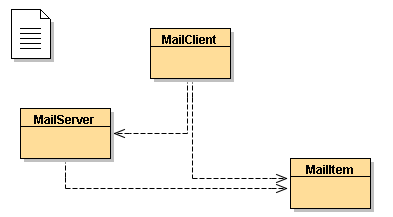
\includegraphics[height=5cm, keepaspectratio]{./figures/mailclass}
\end{center}
\end{frame}

\begin{frame}[fragile]
\frametitle{The this Keyword}
\begin{lstlisting}
public class MailItem
{
	private String from;
	private String to;
	private String message;

  public MailItem(String from, String to, 
                  String message)‏
    {
        this.from = from;
        this.to = to;
        this.message = message;
    }
\end{lstlisting}
\end{frame}

\begin{frame}[fragile]
\frametitle{The this Keyword}
\begin{itemize}
\item \lstinline!this.from = from!
\begin{itemize}
\item \alert{name overloading}: the same name is used for two different entities: instance variable and formal parameter.
\item this is used to go out of the scope of the constructor to class level
\item \alert{\lstinline!this!} always refers to the current object.
\item can also used for methods
\item for internal methods calls and access to instance fields Java automatically inserts this:
\lstinline!updateDisplay -> this.updateDisplay!
\end{itemize}
\end{itemize}
\end{frame}

\begin{frame}[fragile]
\frametitle{Implementing a Test Program I}
\begin{itemize}
\item The purpose on a test program is to verify that one or more methods have been implemented correctly
\item A test program calls methods and checks that they return the expected results. 
\item It contains the following steps:
\begin{enumerate}
\item Provide a tester class
\item Supply a \lstinline!main! method
\item Inside the \lstinline!main! method, create one or more objects
\item Apply methods to the objects
\item Display the results of the method calls - if needed
\item Display the valued that you expect to get - if possible
\end{enumerate}
\end{itemize}
\end{frame}

\begin{frame}[fragile]
\frametitle{Implementing a Test Program II}
\begin{itemize}
\item Consider the Shapes project. It contains allows you to draw circles, squares and triangles on a canvas. 
\item To this extend it contains the classes: Circle, Squares, Triangle and Canvas
\item To test if the implementation is correct we can write a test class
\begin{lstlisting}
public class ShapesTest
{
   public static void main(String[] args)
   {
        Canvas c = Canvas.getCanvas();
        Circle c1 = new Circle();
        Square s1 = new Square();
        Triangle t1 = new Triangle();
        c1.makeVisible();
        s1.makeVisible();
        t1.makeVisible();
        ...
   }
}
\end{lstlisting}
\end{itemize}
\end{frame}

\begin{frame}[fragile]
\frametitle{Implementing Applications}
\begin{itemize}
\item the \lstinline!main! method of your application class should be relatively short
\item normally a few objects are created and a few methods are invoked. 
\item the invoked methods will determine the behaviour of your application.
\end{itemize}
\end{frame}




\end{document}
